\documentclass{article}
\usepackage[left=2cm,right=2cm,top=3cm,bottom=3cm,letterpaper]{geometry}
\usepackage[spanish]{babel}
\usepackage[utf8]{inputenc}
\usepackage{amsmath}
\usepackage{graphicx}

\title{Naive Bayes}
\author{Adolfo Marín Arriaga \and Juan Carlos López López \and Luis Rodrigo Rojo Morales}
\date{\today\\}

\begin{document}
 \maketitle
 
 \begin{itemize}
  \item Clasificadores para la comparación\\
  Para la comparación, los clasificadores Naive Bayes que se usaron son los del archivo NaiveBayes.java que es nuestra implementación y el de la biblioteca e1071 en r.
  \item Primer clasificador\\
  Usando el de NaiveBayes.java para clasificar los elementos que vienen en el archivo AdultDataSetTest.csv nos da el resultado:\\
  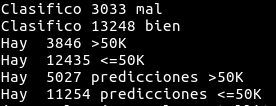
\includegraphics[scale=1]{nbjava}
  \item Segundo clasificador\\
  Usando la biblioteca e1071 de r para clasificar los elementos que vienen en el archivo AdultDataSetTest.csv nos da el resultado:\\
  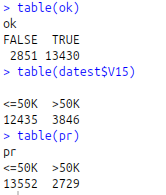
\includegraphics[scale=1]{nbr}\\
  \item Comparación\\
  Lo que nos dicen estos resultados es que hay 12435 personas de la clase $<=$50k y hay 3846 de la clase $>$50k.\\
  El primer clasificador clasificó 11254 personas en la clase $<=$50k y 5027 en la clase $>$50k.\\
  El segundo clasificador clasificó 13552 personas en la clase $<=$50k y 2729 en la clase $>$50k.\\
  El primer clasificador clasificó bien a 13248 personas y mal a 3033 personas.\\
  El segundo clasificador clasificó bien a 13430 personas y mal a 2851 personas.\\
  El primer clasificador acertó en el 81.37\% de los casos.\\
  El segundo clasificador acertó en el 82.49\% de los casos.\\
 \end{itemize}
 
\end{document}
